\section{Lecture 11: Potential Barrier}

Aside: Solving Eigenfunction Problems

There are two problems we are primary interested in:
\begin{enumerate}
    \item $\Psi(\mbf{r}, t)$ is given, find the decomposition into $\sum_E c_E \Psi_E(\mbf{r})$
    \item Tailor the most general solution to a given problem, i.e. find the $c_E$
\end{enumerate}

Now we consider the case of a potential barrier:
\[ V(x) = \begin{cases}
    0 & x < 0 \\ V_0 & 0 < x < a \\ 0 & x > a
\end{cases} \]
By the intuition we build up last time, we see:

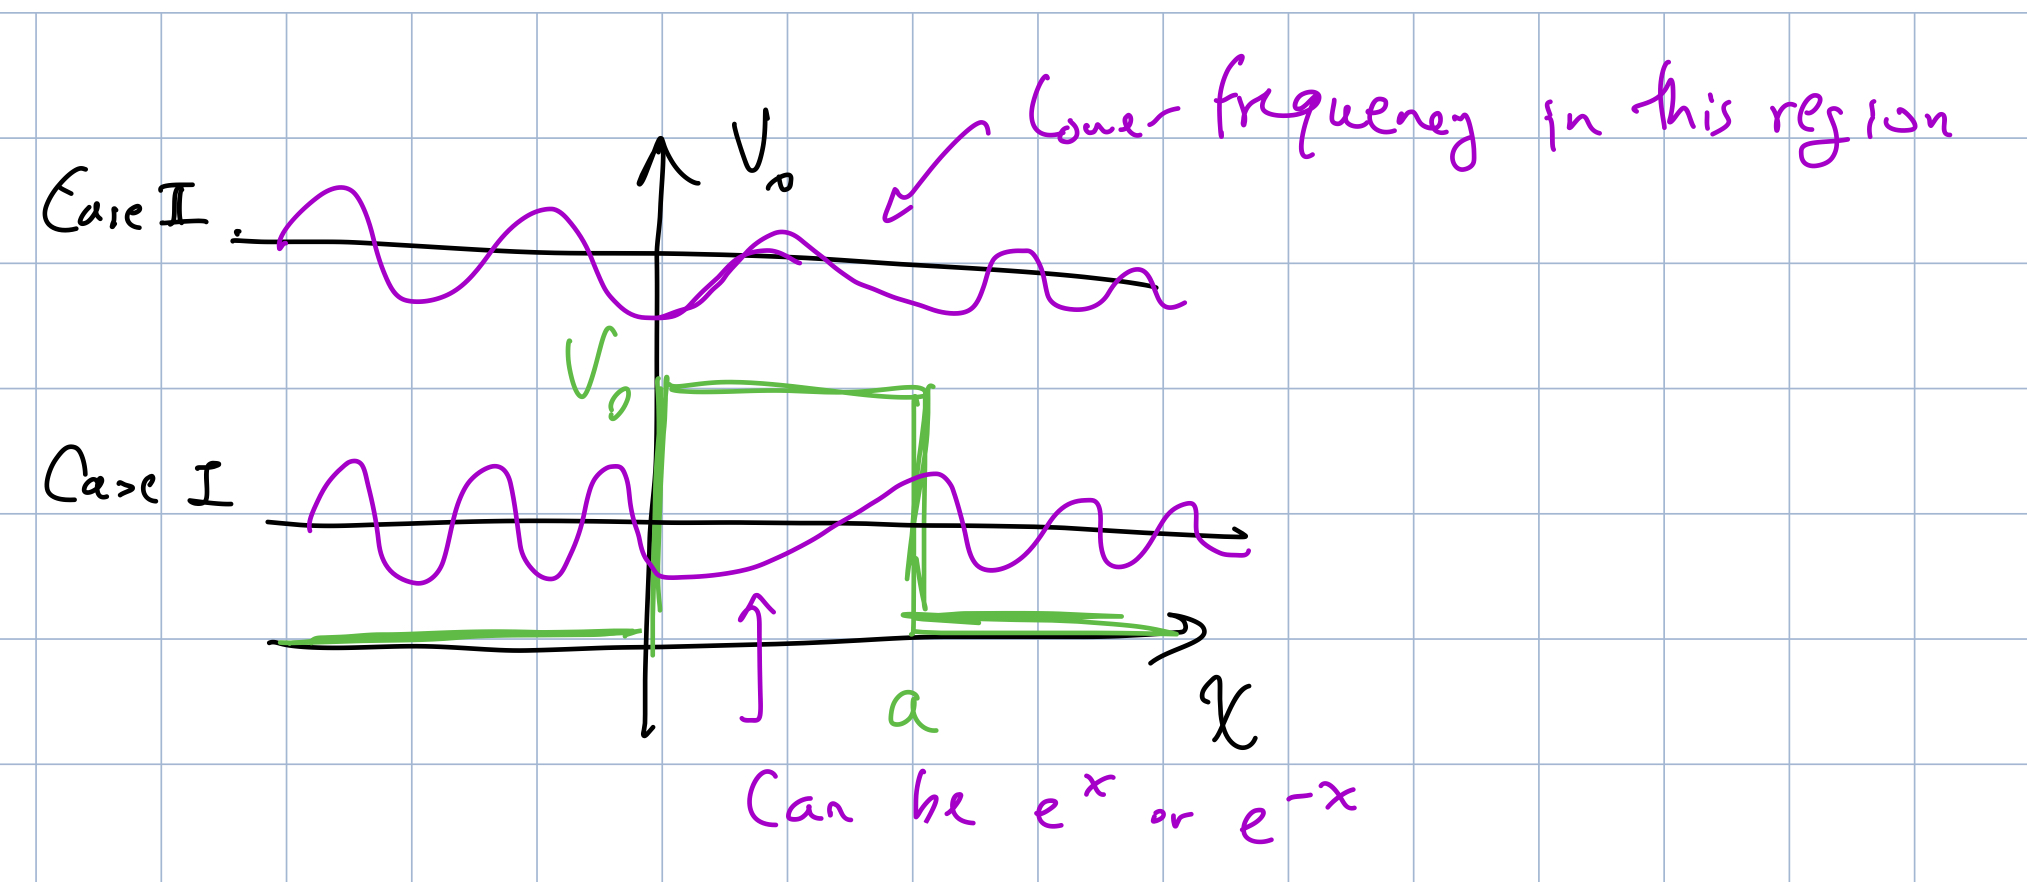
\includegraphics[width=400px]{potbarrier.jpeg}

So our solutions are, with $k = \qty(\frac{2mE}{\hbar^2})^{1/2}$ and $\kappa = \qty(\frac{2m}{\hbar}(V_0 - E))^{1/2}$.
\[ \Psi(x) = \begin{cases}
    Ae^{ikx} + Be^{-ikx} & x < 0 \\
    Fe^{\kappa x} + Ge^{-\kappa x} & 0 < x < a \\
    Ce^{ikx} + De^{-ikx} & x > a
\end{cases} \]
Now let's impose some boundary conditions. Consider a particle incident from the left.

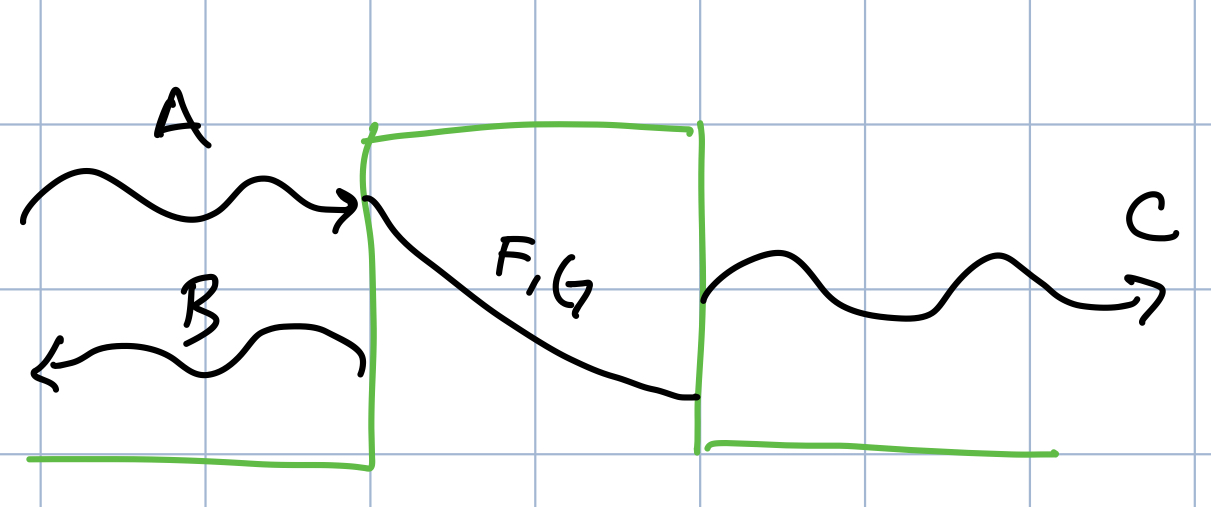
\includegraphics[width=300px]{transbarrier.jpeg}

We do not need to remove $F$ because the positive solution doesn't blow up in the $[0, a]$ region. If we take $v = \frac{\hbar k}{m}$, we
have
\[ \mbf{j} = \begin{cases}
    v[|A|^2 - |B|^2] \\
    v |C|^2
\end{cases} \]
with again:
\[ \mathfrak{R} = \frac{|B|^2}{|A|^2}, \tau = \frac{|C|^2}{|A|^2} \]
Let's match the boundary conditions. At $x = 0$:
\begin{align*}
    \Psi : A + B &= F + G \\
    \Psi' : ik(A - B) &= \kappa(F - G)
\end{align*}
and then at $x = a$:
\begin{align*}
    \Psi : Ce^{ika} &= Fe^{\kappa a} + Ge^{-\kappa a} \\
    \Psi' : ikCe^{ika} &= \kappa(Fe^{ika} - Ge^{ika})
\end{align*}
Our goal is to eliminate $F, G$ to make our lives easier and try doing things in terms of $B/A$ and $C/A$. This yields:
\begin{align*}
    \frac{B}{A} &= \frac{(k^2 + \kappa^2)(e^{2\kappa a} - 1)}{e^{2\kappa a}(k + i \kappa)^2 - (k - i \kappa)^2} \\
    \frac{C}{A} &= \frac{4ik\kappa e^{-ika} e^{\kappa a}}{e^{2\kappa a}(k + i \kappa)^2 - (k - i \kappa)^2} \\
    \mathfrak{R} &= \qty[1 + \frac{4E(V_0 - E)}{V_0^2 \sinh^2(\kappa a)}]^{-1} \\
    \tau &= \qty[1 + \frac{V_0^2 \sinh^2(\kappa a)}{4E(V_0 - E)}]^{-1}
\end{align*}
Note that the transmittance is nonzero, which means some amount of the particle makes it through the potential barrier!
This is the phenomenon known as quantum tunneling. Suppose $\frac{mV_0 a^2}{\hbar^2} = \frac{1}{4}$.

This is the reason fusion is possible. Although there is a Coulomb repulsion between two Hydrogen nuclei, there is a strong force attraction when they are close together.
Instead, it doesn't take as much energy as you actually need to overcome the barrier classically. You can tunnel
below the barrier at some point, so the sun is much colder than classical physics predicts!

Let us Taylor expand the transmittance:
\[ \lim_{E \to V_0} \tau = \qty(1 + \frac{mV_0a^2}{2\hbar})^{-1} \]
where the second term is known as the ``opacity" of the barrier.

Let's take Case II now. The wave is still the same for $x < 0$ and $x > a$ (but $A, B, C, D$ are different).
Instead the barrier we have some $ik'$ instead (similar to last lecture).
\begin{align*}
    \mathfrak{R} &= \qty(1 + \frac{4E(E - V_0)}{V_0^2 \sin^2(k'a)})^{-1} \\
    \tau &= \qty(1 + \frac{V_0^2 \sin^2(k' a)}{4E(E - V_0)})
\end{align*}

Here is the last point of the potential barrier, explaned through pictures. There is a reflection
on both ends of the barrier like so:

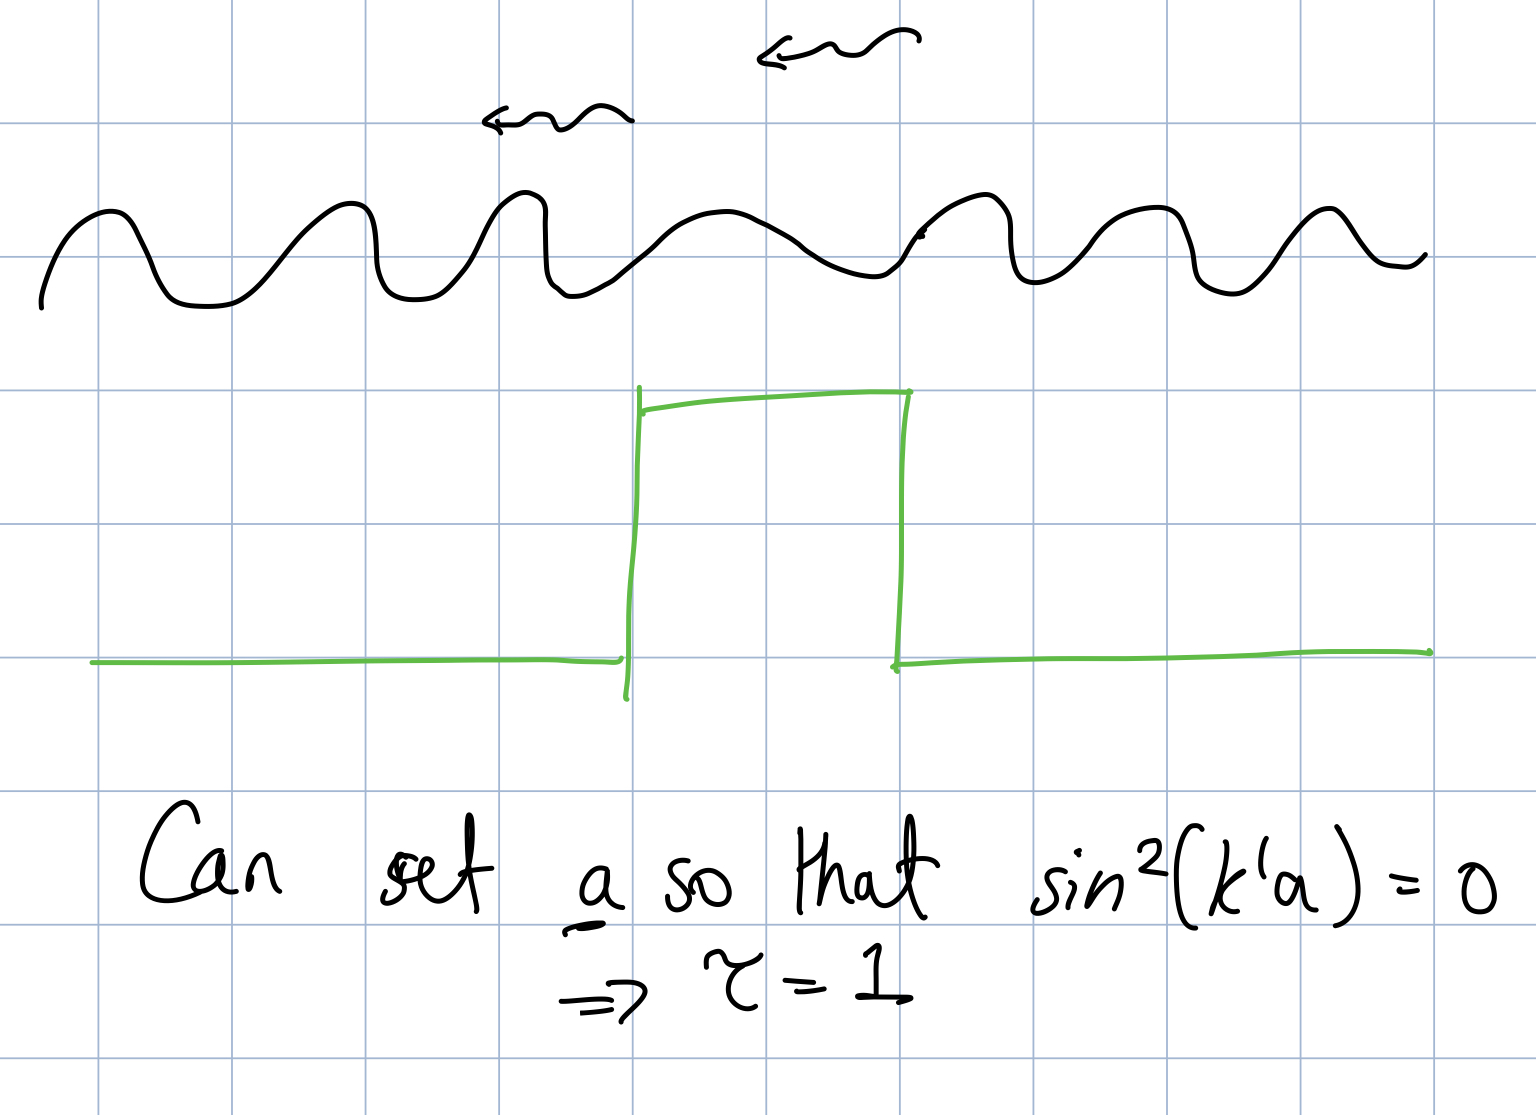
\includegraphics[width=300px]{weirdreflecto.jpeg}

So, if we align the phases perfectly of the two reflections, they cancel and we don't lose any energy.

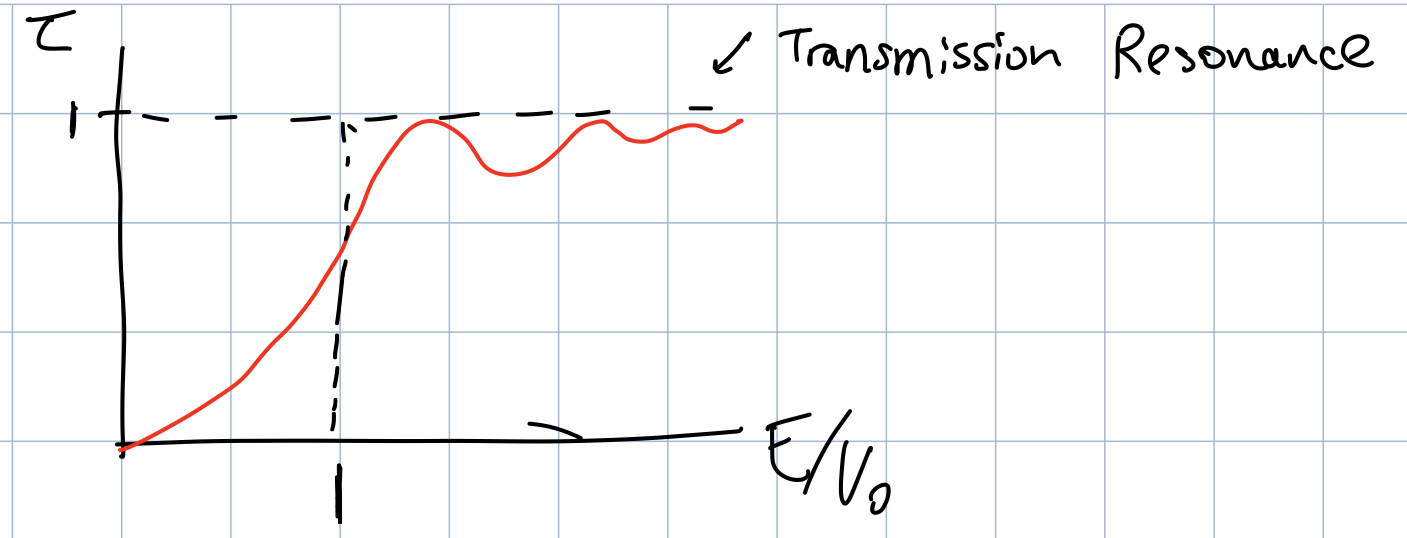
\includegraphics[width=350px]{transres.jpeg}

This is analogous to optics (another wave theory!).

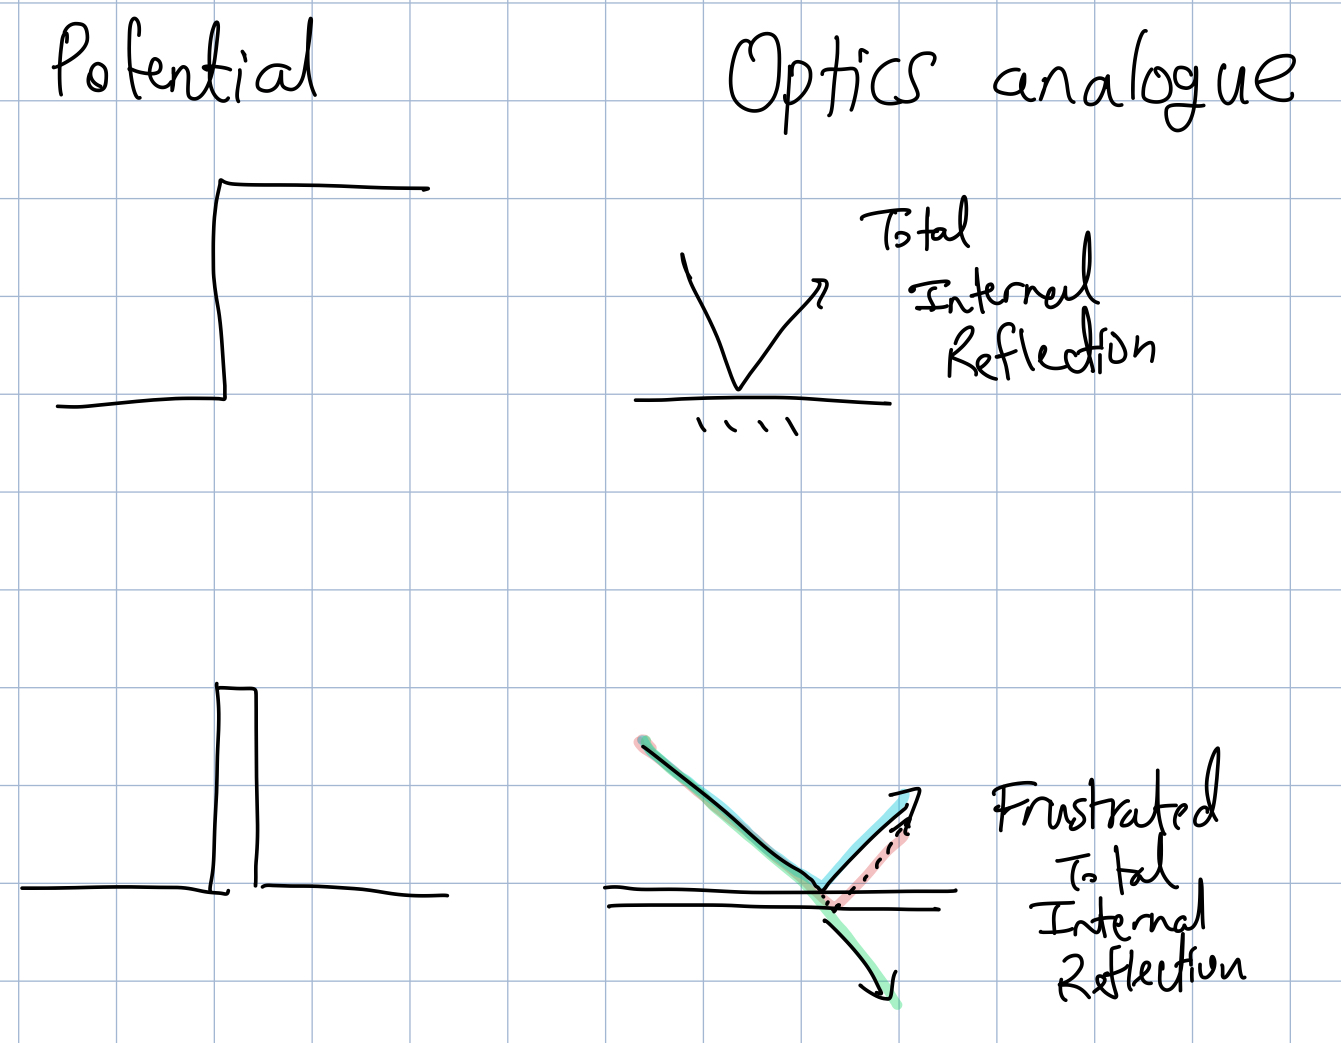
\includegraphics[width=300px]{opticspot.jpeg}